\documentclass[a4paper]{article}
%\usepackage{a4wide} % márgenes un poco más anchos que lo usual


\usepackage[spanish]{babel} % Le indicamos a LaTeX que vamos a escribir en español.
\usepackage[utf8]{inputenc} % Permite utilizar tildes y eñes normalmente
\usepackage{caratula} % Se puede descargar en ~> https://github.com/bcardiff/dc-tex
\usepackage[breaklinks=true]{hyperref}
\usepackage{float}


\begin{document} % Todo lo que escribamos a partir de aca va a aparecer en el documento.


\begin{figure}[H] 
\centering
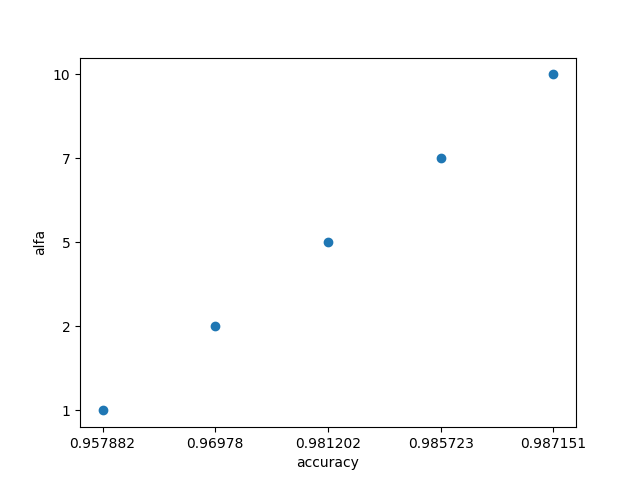
\includegraphics[width=1\textwidth]{img/big_alfa_pca_accu.png}
\caption{Accuracy en función de alfa, Knn+PCA}
\label{fig:big_alfa_pca_accu}
\end{figure}



\begin{figure}[H] 
\centering
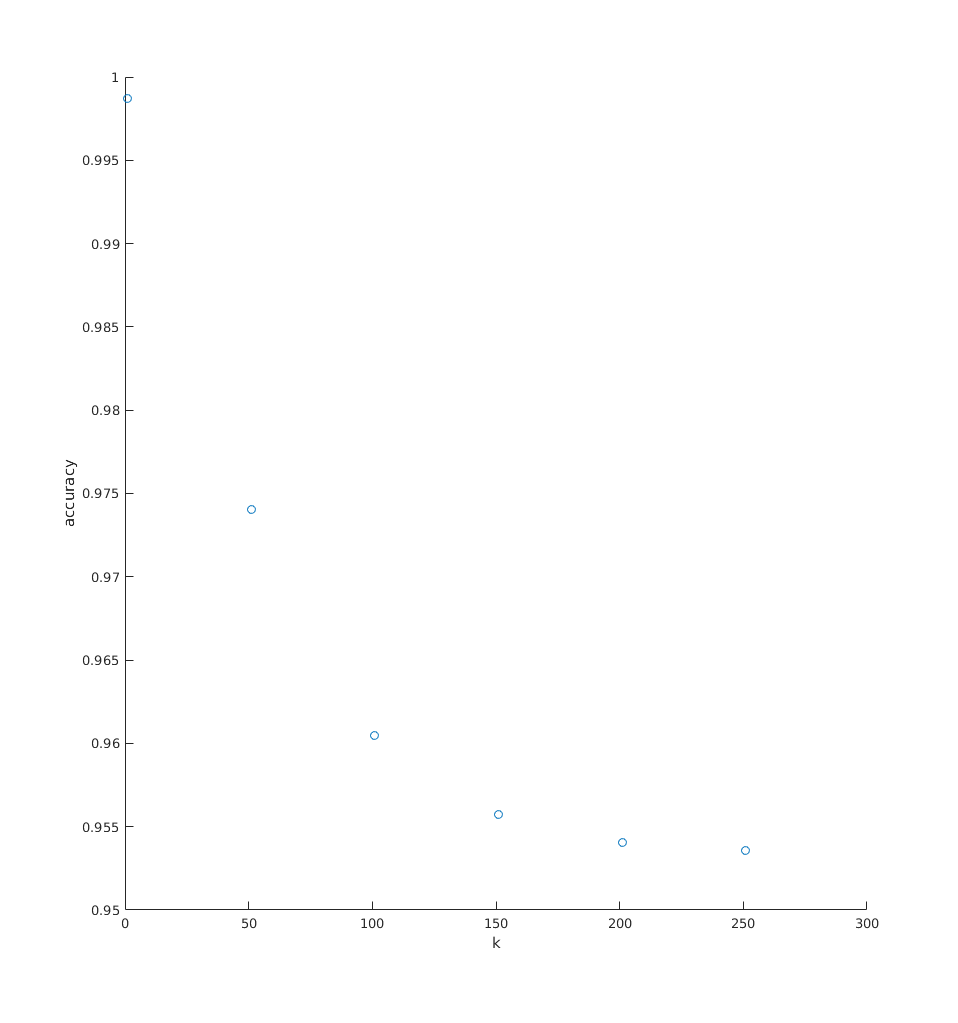
\includegraphics[width=1\textwidth]{img/big_k_knn_accu.png}
\caption{Accuracy en función de K, Knn}
\label{fig:big_k_knn_accu}
\end{figure}

\begin{figure}[H] 
\centering
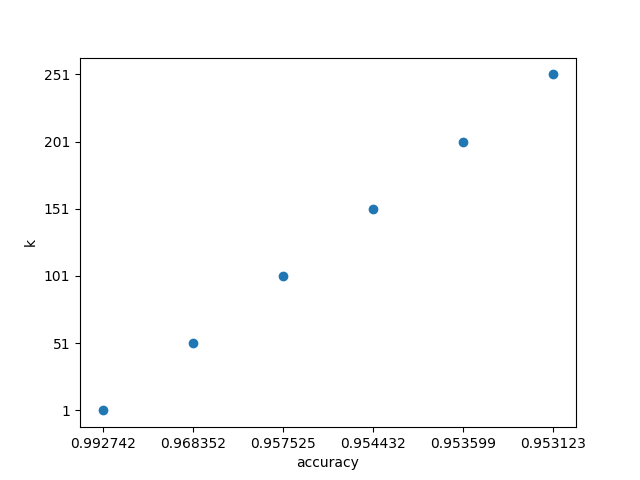
\includegraphics[width=1\textwidth]{img/big_k_pca_accu.png}
\caption{Accuracy en función de K, Knn+PCA}
\label{fig:big_k_pca_accu}
\end{figure}


\begin{figure}[H] 
\centering
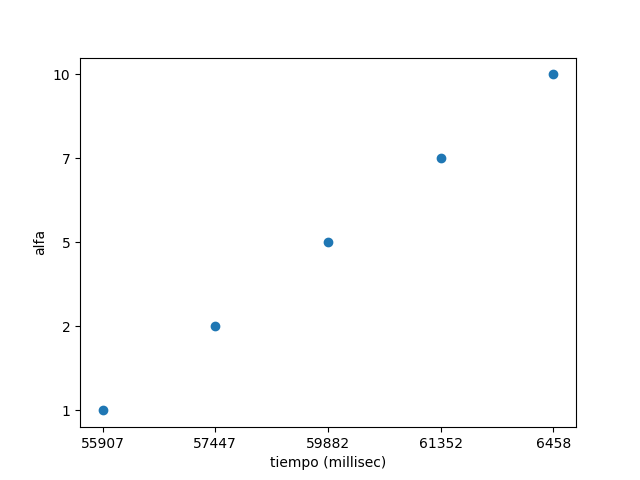
\includegraphics[width=1\textwidth]{img/big_alfa_pca_tiempo.png}
\caption{Tiempo en función del alfa, Knn+PCA}
\label{fig:big_alfa_pca_tiempo}
\end{figure}


\begin{figure}[H] 
\centering
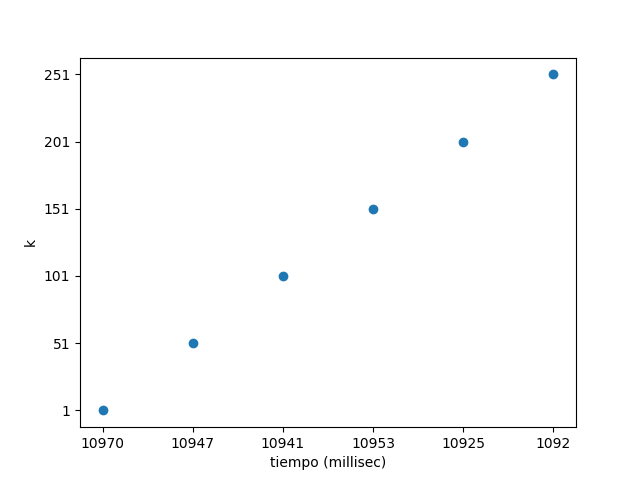
\includegraphics[width=1\textwidth]{img/big_k_knn_tiempo.png}
\caption{Tiempo en función de K, Knn}
\label{fig:big_k_knn_tiempo}
\end{figure}

\begin{figure}[H] 
\centering
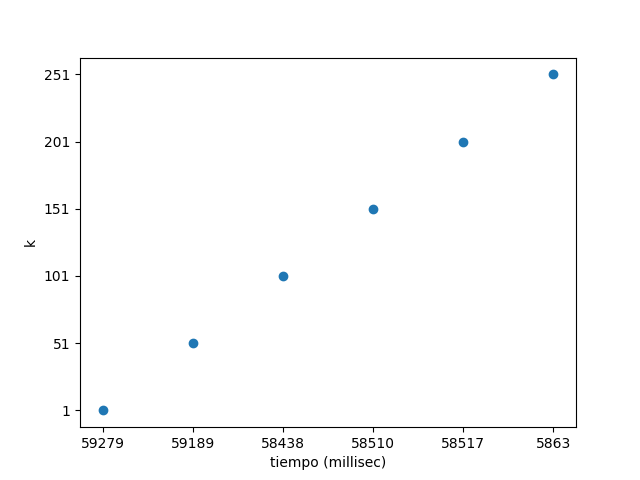
\includegraphics[width=1\textwidth]{img/big_k_pca_tiempo.png}
\caption{Tiempo en función de K, Knn+PCA}
\label{fig:big_k_pca_tiempo}
\end{figure}



\end{document}

